%!TeX root=../Dissertation.tex
%!TeX bibfile=./synthesis.bib

\chapter{System creation and setup}
\section{The host machine}
\subsection{Hardware}
It was decided as a better test of Docker's ability to reduce strain on a system, that an older machine with limited resources would be used rather than a more modern and capable machine. This was to better represent the target group of this research; that being SMEs that may have aging hardware, attempting to get the most out of what they currently have available.

The test machine has %TODO: TO DO state what the specs of the machine are. RAM, CPU, etc

\subsection{Operating System}

\section{Servers}
\subsection{Operating system}
Both systems were created from scratch, using the latest LTS versions of Ubuntu Server (20.04, Focal Fossa Server \citep{UbuntuServerDocumentation}).

For VMware, the images were downloaded directly from the Ubuntu Website and the virtual machines were created using VMware's workstation Virtual Machine creation wizard, whereas for Docker, the Ubuntu Server image was taken from Ubuntu's official Docker Image, hosted on Docker Hub \citep{UbuntuDockerHub}. Each docker image was then created using a Dockerfile, which lays out which version to use; in this case, ubuntu:latest.

\subsection{Software}
The servers were created to use the software and topology laid out in the requirements within section \ref{Requirements:infrastructure}.

For both VMware and Docker this meant using the Advanced Package Tool (which is the default package manager on ubuntu) to install the various software needed.

However, for VMware this was done once each server was installed and booted. On Docker, through the use of Dockerfiles, this can integrated directly into the Docker image, along with any configuration files that may be required, such as local zone files for the primary DNS server (DNS1). An example of a Dockerfile for DNS1 is shown in figure \ref{fig:dockerfileexample} below. This shows how the base image is selected, along with the addition of the software and tools necessary to make bind9 work. The `COPY' command takes the completed configuration files and places them in the correct folders.
%\begin{figure}[h]
%\caption{}
%\label{fig:dockerfileexample}
%\begin{minted}{dockerfile}
%FROM ubuntu:latest
%
%RUN apt-get update \
%  && apt-get install -y \
%  bind9 \
%  bind9utils \
%  bind9-doc
%
%
%COPY named.conf.options /etc/bind/
%COPY named.conf.local /etc/bind/
%COPY db.intranet.co.uk /etc/bind/
%COPY db.72.168.192.in-addr.arpa /etc/bind/
%
%CMD ["/bin/bash", "-c", "while :; do sleep 10; done"]
%
%\end{minted}
%
%\end{figure}

\section{Client}
\subsection{Operating System}
\label{ClientOS}
The client machine was created using VMware workstation pro, using Ubuntu's latest LTS desktop version (20.04, Focal Fossa Desktop \citep{UbuntuDesktopDocumentation})

The same client machine was used for both the VMware system and the Docker System. This was to ensure that the client used the same amount of resources (RAM, CPU and Network usage) on the host machine for both the VMware tests and the Docker tests, as in a real environment, the clients would be remote devices on the network. By using the same virtual machine as the client in both tests, any impact to the outputs of the tests should be mitigated.

The Client machine was configured to use up to 4GB of RAM, and up to two cores using VMware Workstation Pro.

\subsection{Software}
The client machine had all the testing and benchmarking software required installed before any testing took place, so that the machine was the same between testing.

The software installed was as described in the requirements list in section \ref{RequirementsListBench}. As mentioned in that section, Netdata is installed on the host machine during the final test, not the client machine. This is to ensure that usage statistics represent the whole machine, not just the client, or the endpoint (in this case, the web server).

\section{The Network}
For both tests, VMware Workstation's NAT networking mode was used \citep{VMwareNAT}. The same network was used for both in order to ensure a fair test. Using the same network provided by VMware's NAT setting ensures that any differences in network performance measured in the tests is due to factors other than the network infrastructure itself; more specifically, the difference between Docker and VMware's core performance in a network setting.

The configuration of this network was edited using VMware's "Virtual Network Settings" \citep{VMwareNetChange} to disable the built in DHCP server, so that it didn't conflict with the DHCP server created for the testing (see subsection \ref{DHCP Spec}).

Setting up VMware Virtual Machines to use the NAT (VMnet8) network is straight-forward. On the contrary, to do the Docker test, more work was required. Firstly, a Custom Docker Network named "CustomNet" was set up using Docker's "macvlan" network driver \citep{DockerMacVlan}. This network driver is designed to be bound to a physical network, similar to the "bridged" mode found in VMware, by giving each Container an individual MAC address. When creating a "macvlan" network, the interface to be used must be specified. This is where VMware's Virtual Network Adapter was used \citep{VMwareNetworkAdapter}, which is designed to allow the host machine to communicate with virtual machines over a virtualised IP interface that installed on the host machine. This allowed the Docker Network "CustomNet" to be bound to the VMnet8 interface, thus allowing the Docker containers to communicate with each other over the VMware network. This also made it possible for the VMware client to be used in the Docker test as explained in subsection \ref{ClientOS}.

Table \ref{tab:IPaddressing} shows the IP addressing and hostname scheme that was used in both tests.

\begin{table}[H]
\caption{}
\label{tab:IPaddressing}
\centering
\resizebox{\textwidth}{!}{%
\begin{tabular}{|l|l|l|}
\hline
 & \textbf{IP Address} & \textbf{DNS Hostname} \\ \hline
\textbf{DNS1} & 192.168.72.3/24 & No hostname \\ \hline
\textbf{DNS2} & 192.168.72.4/24 & ns1.intranet.co.uk \\ \hline
\textbf{DNS3} & 192.168.72.5/24 & ns2.intranet.co.uk \\ \hline
\textbf{DHCP} & 192.168.72.6/24 & dhcp.intranet.co.uk \\ \hline
\textbf{Apache} & 192.168.72.150 & www.intranet.co.uk \\ \hline
\textbf{MySQL} & 192.168.72.151 & mysql.intranet.co.uk \\ \hline
\textbf{Client Addresses} & 192.168.72.50/24 - 192.168.72.100/24 & No hostname \\ \hline
\end{tabular}%
}
\end{table}

For testing, when a server needed to be specified, the hostname was used over the IP address where applicable so that the process would make use of the DNS infrastructure. For example, 'www.intranet.co.uk' is used in the Jmeter test, instead of '192.168.72.150'.



\chapter{Methods}



\chapter{Testing \& Benchmarks}
Introductory explanations for each of these tests and benchmarks are included in the requirements in section \ref{RequirementsListBench}.

\section{Test 1 - iPerf3 Throughput}
\subsection{Test parameters}
In this test, the throughput is measured between the Apache server and the Client. The listener for iPerf3 was setup on the Apache server using port 5201 (the default port for iPerf3 \citep{iPerf3Documentation}). The client then specifies that is is in-fact running iPerf3 as a client, and tells the server which format to record throughput with. For this testing, the format used was 'M', meaning Megabytes \citep{iPerf3Documentation}.

The test runs for ten seconds, taking measurements of total throughput in a second, resulting in ten points that can be converted into a graph showing the transfer rate (throughput) over time in Megabytes per second. An average can also be taken from this. A separate throughput is calculated on each side of the transaction (at the server, and at the client).
 
\subsection{Results}
The average throughputs for both tests, and for clients and severs, are shown in table \ref{tab:iperf3average} below.

\begin{table}[h]
\centering
\caption{Table showing the average transfer rate in a 10 second period}
\label{tab:iperf3average}
\resizebox{\textwidth}{!}{%
\begin{tabular}{|c|c|c|}
\hline
x & \textbf{VMware Average (MBytes/s)} & \textbf{Docker Average (MBytes/s)} \\ \hline
\textbf{Client} & 176.37 & 290.70 \\ \hline
\textbf{Apache Server} & 172.61 & 290.40 \\ \hline
\end{tabular}%
}
\end{table}

The averages shown in this table clearly show a higher throughput for the Docker system, with an improvement (averaged between the Client and the Apache Server) of 116.06 MegaBytes per Second.

Figure \ref{fig:test1graphs} shows the transfer rate over time for both Client and Server.

\begin{figure}[H]
\caption{}
\label{fig:test1graphs}
\fbox{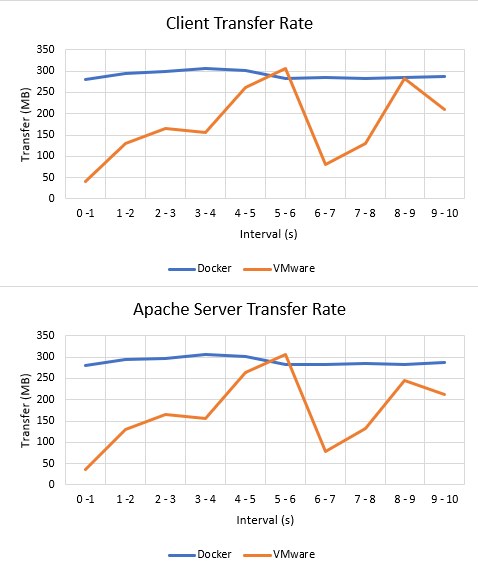
\includegraphics[width=0.8\textwidth]{./synthesis/test1graphs.PNG}}
\centering
\end{figure}

This shows that Docker is stable, whilst VMware's throughput result fluctuates far more. This would suggest that the VMware system is unstable; something we will investigate further in the evaluation section of this report.

\section{Test 2 - Sysbench MySQL Input/Output}
\subsection{Test parameters}
This test required a test database with random data to be created on the MySQL server. Luckily, Sysbench includes a 'prepare' tool, which allows a user to specify parameters of for the table that match the test they want to conduct \citep{sysbench}. Sysbench then creates, or \emph{prepares}, a database that is suitable for said test. A test user account with all permissions was also created for Sysbench to use. When the prepare command is run, it creates the database and tables, and then fills the tables with the amount ant type of data specified.

The database we created for testing had the following parameters:
\begin{itemize}
  \item The database had two tables.
  \item Each table had a size of 500000.
  \item Table size in sysbench relates to rows. Meaning across the two tables, there was a total of one million rows of data.
  \item The test was specified as '\texttt{oltp\_read\_write}'.
\end{itemize}

OLTP is Online Transaction Processing\citep{oltp}, which is a term used to describe online databases that generally have high throughput and connectivity from many users \citep{oracleoltp}. The \texttt{oltp\_read\_write} test attempts to simulate an OLTP workload by performing various different SELECT, DELETE, INSERT and UPDATE queries on the data \citep{sysbenchmarking}.

Once the above table was created, the actual test could be performed. The client machine runs the command that starts the test, and the domain name for the MySQL server (mysql.intranet.co.uk) was used to specify where the server and database were located.

The test was run using the following parameters:
\begin{itemize}
  \item The port was set as 3306 (the default for MySQL).
  \item Two threads were used. This simulates the database being accessed and changed by two different users or programs at the same time.
  \item 'Time' was set as 300. This is in seconds, meaning the scenario ran for five minutes.
  \item 'Events' was set as 0. This setting would allow the user to specify that the test should stop after a certain number of events have been reached. By setting this to '0', the test will continue to run until the 'Time' setting is reached.
\end{itemize}
\subsection{Results}
\label{test2results}

Figure \ref{fig:test2fiveminutes} shows the total number of Read, Write and Other queries performed by Sysbench in a 5 minute period. The results for both systems are compared side by side.

This graph shows a clear win for Docker, with the VMware system managing to perform just over a third of the number of Reads that Docker managed in the same time frame.

\begin{figure}[H]
\caption{}
\label{fig:test2fiveminutes}
\fbox{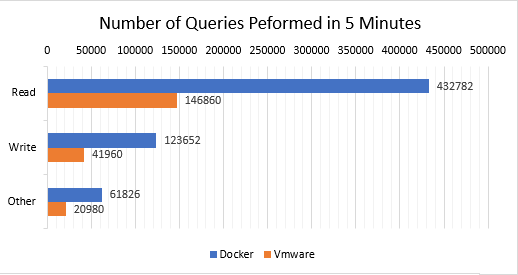
\includegraphics[width=\textwidth]{./synthesis/test2fivemingraph.png}}
\centering
\end{figure}

Figure \ref{fig:test2onesecgraph} shows both the total queries per second, and the total transactions per second for both systems. A query is defined as being a single statement such as SELECT, INSERT or UPDATE\citep{mysqlqueries}; whereas a transaction is a combination of multiple of these statements within one command\citep{mysqltransactions}, typically in order to manipulate multiple rows of data.

This further shows just how much faster the Docker system was at data manipulation.

\begin{figure}[H]
\caption{}
\label{fig:test2onesecgraph}
\fbox{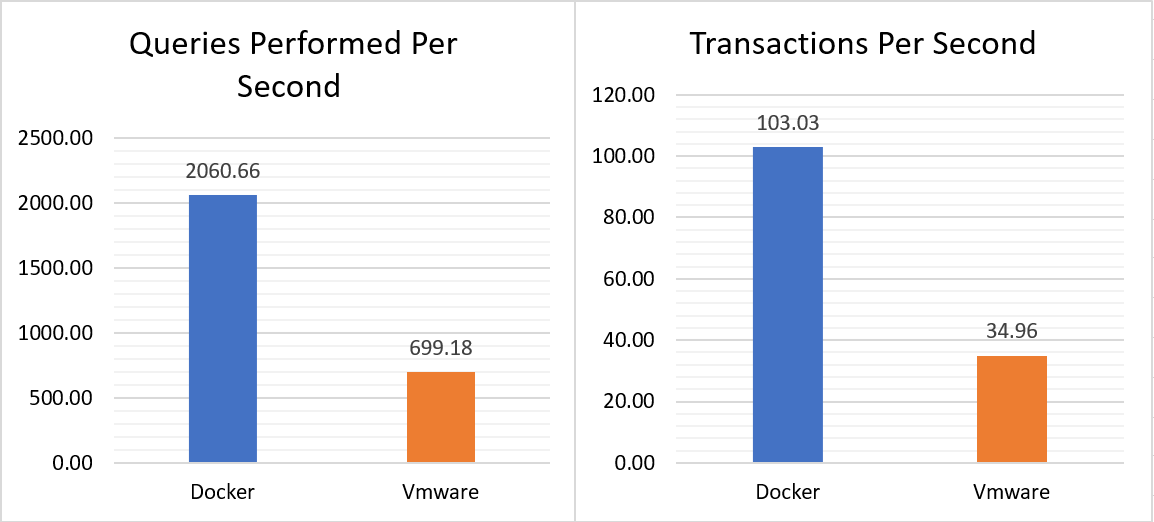
\includegraphics[width=\textwidth]{./synthesis/test2onesecgraph.PNG}}
\centering
\end{figure}

The latency between queries was also measured by Sysbench. Figure \ref{test2latencygraph} shows a latency bar graph, with the minimum, average, and 95th percentile latencies in Milliseconds. The 95th percentile was rather than the maximum, because both tests experienced a maximum latency that would have dwarfed the other results. These maximum latencies were also most likely errors (which were to be expected with such a high number of queries being performed \citep{oltp}).

\begin{figure}[H]
\caption{}
\label{test2latencygraph}
\fbox{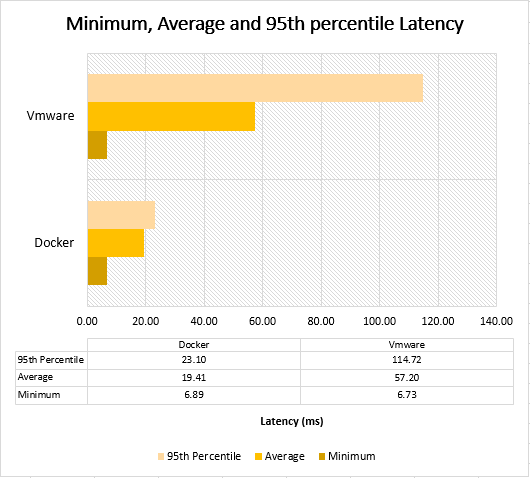
\includegraphics[width=0.90\textwidth]{./synthesis/test2latencygraph.PNG}}
\centering
\end{figure}

We can see from these results, that Docker far out performs VMware in terms of latency, to such an extreme extent that Dockers' top 95th percentile results are lower than VMware's average latency.

\section{Test 3 - Namebench}
\subsection{Test parameters}
This test compares the performance of the DNS servers and their ability to perform DNS queries for various websites.

Namebench works by going through a list (specified by the user) of websites and recording the latency for the DNS server to perform the query\citep{Namebench}. Before the test commenced, the caches on all of the DNS servers in our infrastructure were wiped to ensure a fair test between the two systems. In our testing, the following parameters were set:
\begin{itemize}
  \item The list to be used was specified as 'alexa'. This option uses Amazon's Alexa Top Sites list \citep{alexainternet}. Around 38,000 different website addresses were tested. Having a high number of tests is important because it gives a good average.
  \item Both DNS2 and DNS3 were specified (using their domain names: ns1.intranet.co.uk and ns2.intranet.co.uk respectively) to be tested. DNS1 is a primary server, and is hidden in the network topology, only to be used as the master for the 'intranet.co.uk' domain, so it isn't tested here.
\end{itemize}

\subsection{Results}
Figure \ref{fig:test3graphaverage} shows a graph of the average DNS response times. We can see from this graph that Docker has smaller average DNS response when compared to VMware. An interesting, but unrelated behaviour here is that DNS2 in both tests out performed DNS3; this is unexpected given that both servers share exactly the same configuration. Perhaps this is a characteristic of the way that BIND9 handles secondary DNS servers?

\begin{figure}[H]
\caption{}
\label{fig:test3graphaverage}
\fbox{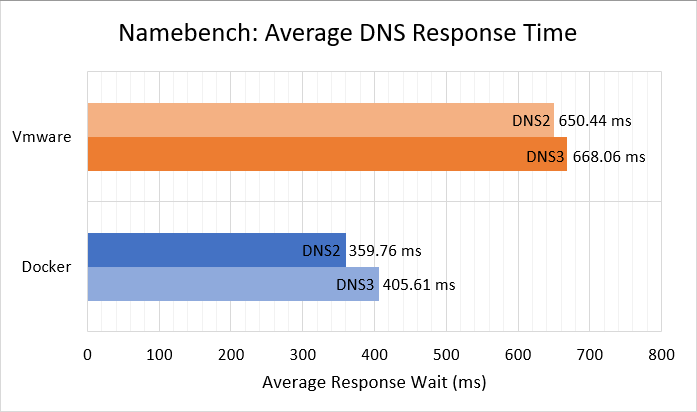
\includegraphics[width=0.8\textwidth]{./synthesis/test3graphaverage.PNG}}
\centering
\end{figure}

We can see the minimum latency response in figure \ref{fig:test3graphmin}. Here, Docker takes the win again, with a similar relative margin between results as with the average latency shown above. Here we can see that the latency for each server is the same within the same system; this helps us to rule out an element of chance to the results (ie, the results are more likely to be genuine given that they are the same across the two severs for the same system).

\begin{figure}[H]
\caption{}
\label{fig:test3graphmin}
\fbox{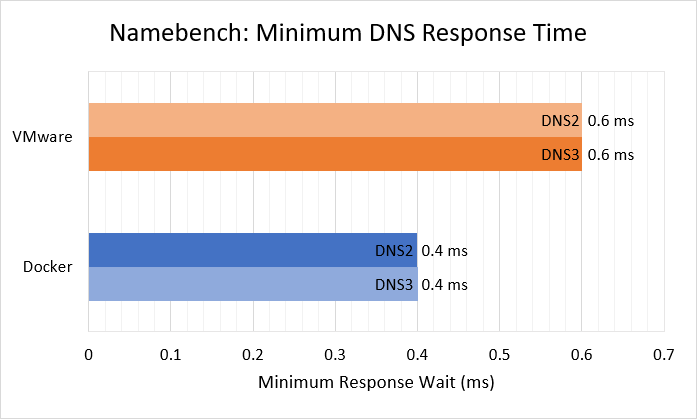
\includegraphics[width=0.8\textwidth]{./synthesis/test3graphmin.PNG}}
\centering
\end{figure}

No maximum latency is given in a graph as in both tests, certain requests hit their maximum wait time for a response (3500ms). This is most likely due to an error with authoritative servers outside of our control. Furthermore, 95th percentile data could not be used (such as in our last test in subsection \ref{test2results}) because Namebench compiles the the minimum, average and maximum data itself, without allowing the user to access raw data. (Most likely because the domain name list provided by Alexa \citep{alexainternet} is propriety, so providing access to this data could be a breach of Alexa's agreements.

\section{Test 4 - Apache JMeter and Performance measurements using Netdata}
\subsection{Test parameters}
%the idle benchmarks didn't have the client machine running!
This test is slightly different, in that the data we get back from the workload isn't the most important piece of data we receive by doing the test. Instead, we are using the workload that is generated using JMeter \citep{ApacheJMeter}, in order to measure the stress on the machine. The three areas of Computing performance we will be looking into here are the CPU usage, RAM usage and the 'Load' on the machine. These were measured using Netdata\citep{Netdata}, so that the data could be monitored on another PC without affecting the performance of the PC running the Containers and Virtual Machines. Netdata also creates real-time graphs that can can then be saved in snapshots, so that we can investigate the results in depth.



Idle data was also

\subsection{Results}
\subsubsection{Jmeter}

\subsubsection{Netdata}
Whilst CPU and RAM usage are self explanatory, 'load' may seem more vague. Load, as measured and defined by Netdata is 